\renewcommand{\thesection}{\arabic{section}}\renewcommand{\theHsection}{chapter.\arabic{section}}\setcounter{section}{1}\section{函数的连续性}
\noindent\begin{minipage}{\textwidth}\ProblemHeading{例题}{2.1（改写）}
设 $A=\{\text{甲},\text{乙},\text{丙}\}$，$B=\{X,Y,Z\}$。分别判断下列规则是否定义了从 $A$ 到 $B$ 的映射，并写出值域：
\SubQ{1}{$f(\text{甲})=X$，$f(\text{乙})=Y$，$f(\text{丙})=Z$。}
\SubQ{2}{$f(\text{甲})=f(\text{乙})=f(\text{丙})=Y$。}
\end{minipage}\par\vfill
\noindent\begin{minipage}{\textwidth}\ProblemHeading{例题}{2.2（改写）}
说明为什么从正整数集 $\mathbb N^*$ 到 $\mathbb R$ 的映射与实数列一一对应，并分别写出从映射得到数列、从数列得到映射的方法。
\end{minipage}\par\vfill
\noindent\begin{minipage}{\textwidth}\ProblemHeading{例题}{2.3（改写）}
规则 $f(x)=\sqrt{1-x^2}$ 是否定义了从 $[-1,1]$ 到 $\mathbb R$ 的映射？说明理由并求其值域。
\end{minipage}\par\vfill
\newpage
\noindent\begin{minipage}{\textwidth}\ProblemHeading{例题}{2.4（改写）}
有 $n$ 位顾客 $A_1,\ldots,A_n$，每人抽取一张标有 $1,\ldots,n$ 中某个号码的彩票，每个号码恰好出现一次。号码 $i$ 对应奖品 $I_i$。以 $g$ 表示顾客到彩票号码的映射，$f(i)=I_i$，$h$ 表示顾客到所得奖品的映射。写出 $g,f,h$ 的定义域、对应规则及 $h$ 与 $f,g$ 的复合关系。
\end{minipage}\par\vfill
\noindent\begin{minipage}{\textwidth}\ProblemHeading{例题}{2.5（改写）}
设 $g(x)=x^2+3x-2$，$f(x)=\sqrt{2+\cos x+\sin x}$，二者定义域均为 $\mathbb R$。求复合函数 $f\circ g$ 的表达式和定义域。
\end{minipage}\par\vfill
\noindent\begin{minipage}{\textwidth}\ProblemHeading{例题}{2.6（改写）}
设 $f(x)=ax+b$，$a\ne0$。用 $f^{\circ n}$ 表示 $f$ 的 $n$ 次复合，证明\[f^{\circ n}(x)=a^nx+(a^{n-1}+\cdots+a+1)b.\]
\end{minipage}\par\vfill
\newpage
\noindent\begin{minipage}{\textwidth}\ProblemHeading{习题}{2.7}
设 $A=\{a,b,c,d\}$。证明存在唯一映射 $f:A\to A$，同时满足 $f(a)=b$、$f(c)=d$，以及对所有 $x\in A$ 有 $f(f(x))=x$。
\end{minipage}\par\vfill
\noindent\begin{minipage}{\textwidth}\ProblemHeading{习题}{2.8}
设自映射 $f$ 满足 $f(f(a))=a$。求 $f^{\circ n}(a)$，其中 $f^{\circ n}$ 表示 $n$ 次复合。
\end{minipage}\par\vfill
\noindent\begin{minipage}{\textwidth}\ProblemHeading{习题}{2.9}
设 Dirichlet 函数 $D(x)=\begin{cases}1,&x\in\mathbb Q,\\0,&x\notin\mathbb Q.\end{cases}$，回答下列问题：
\SubQ{1}{求 $D\circ D$。}
\SubQ{2}{求集合的原像 $D^{-1}(\{0\})$、$D^{-1}(\{1\})$、$D^{-1}(\{0,1\})$。}
\end{minipage}\par\vfill
\newpage
\noindent\begin{minipage}{\textwidth}\ProblemHeading{习题}{2.10}
设 $A$ 有 $n$ 个元素，单射 $f:A\to A$ 称为 $A$ 的一个排列。
\SubQ{1}{证明 $f(A)=A$。}
\SubQ{2}{证明逆映射 $f^{-1}$ 存在。}
\SubQ{3}{$A$ 共有多少个排列？}
\end{minipage}\par\vfill
\noindent\begin{minipage}{\textwidth}\ProblemHeading{习题}{2.11}
设 $A$ 有 $n\ge2$ 个元素。证明存在非恒等排列 $f:A\to A$，使 $f\circ f$ 为恒等排列。
\end{minipage}\par\vfill
\noindent\begin{minipage}{\textwidth}\ProblemHeading{例题}{2.12（改写）}
证明整数集 $\mathbb Z$ 可数，并明确给出 $\mathbb N^*$ 与 $\mathbb Z$ 之间的一个双射。
\end{minipage}\par\vfill
\newpage
\noindent\begin{minipage}{\textwidth}\ProblemHeading{例题}{2.13}
证明开区间 $(0,1)$ 与闭区间 $[0,1]$ 等势。
\end{minipage}\par\vfill
\noindent\begin{minipage}{\textwidth}\ProblemHeading{习题}{2.14}
在平面直角坐标系中，两坐标均为有理数的点称为有理点。证明平面上所有有理点组成的集合可数。
\end{minipage}\par\vfill
\noindent\begin{minipage}{\textwidth}\ProblemHeading{习题}{2.15}
若复数 $x$ 满足某个多项式方程 $a_0x^n+a_1x^{n-1}+\cdots+a_n=0$，其中系数均为整数且 $a_0\ne0$，则称 $x$ 为代数数。证明全体代数数构成可数集。
\end{minipage}\par\vfill
\newpage
\noindent\begin{minipage}{\textwidth}\ProblemHeading{习题}{2.16}
设 $A$ 为实轴上互不相交的非退化区间所组成的集合（$A$ 的元素是区间）。证明 $A$ 至多可数。
\end{minipage}\par\vfill
\noindent\begin{minipage}{\textwidth}\ProblemHeading{习题}{2.17}
设 $S=\{(x_1,x_2,\ldots):x_i\in\{0,1\}\}$。证明 $S$ 与 $[0,1]$ 等势。
\end{minipage}\par\vfill
\noindent\begin{minipage}{\textwidth}\ProblemHeading{习题}{2.18（校订）}
用对角线法证明 $\mathbb R$ 不可数。为避免二进制展开不唯一的问题，使用三进制中仅含数字 $0,2$ 的展开：
\SubQ{1}{证明不同的 $0,2$ 数字序列给出不同的数 $\sum_{j=1}^\infty d_j3^{-j}\in[0,1]$。}
\SubQ{2}{若这些数可列为 $x_1,x_2,\ldots$，写出各自的数字 $d_{ij}$，令 $a_k=2-d_{kk}$。证明数 $x=\sum_{k=1}^\infty a_k3^{-k}$ 不在此列中，从而导出矛盾。}
\end{minipage}\par\vfill
\newpage
\noindent\begin{minipage}{\textwidth}\ProblemHeading{习题}{2.19}
证明可数条直线不能覆盖整个平面。
\end{minipage}\par\vfill
\noindent\begin{minipage}{\textwidth}\ProblemHeading{例题}{2.20（改写）}
有10种产品，编号为 $1,2,\ldots,10$，第 $i$ 种产品的价格为实数 $x_i$。说明对应关系 $f(i)=x_i$ 为什么是函数，并指出其定义域和值域。
\end{minipage}\par\vfill
\noindent\begin{minipage}{\textwidth}\ProblemHeading{例题}{2.21（改写）}
求函数 $f(x)=\sqrt{\frac{1+x}{1-x}}$ 的定义域。
\end{minipage}\par\vfill
\newpage
\noindent\begin{minipage}{\textwidth}\ProblemHeading{例题}{2.22（改写）}
图中给出了某日正午12时至下午6时的气温随时间变化的曲线，横坐标 $t$ 为时刻，纵坐标 $T$ 为气温。说明它为什么定义了一个函数，写出其定义域，并说明若要读出气温的具体数值，还需要怎样的刻度信息。
\begin{center}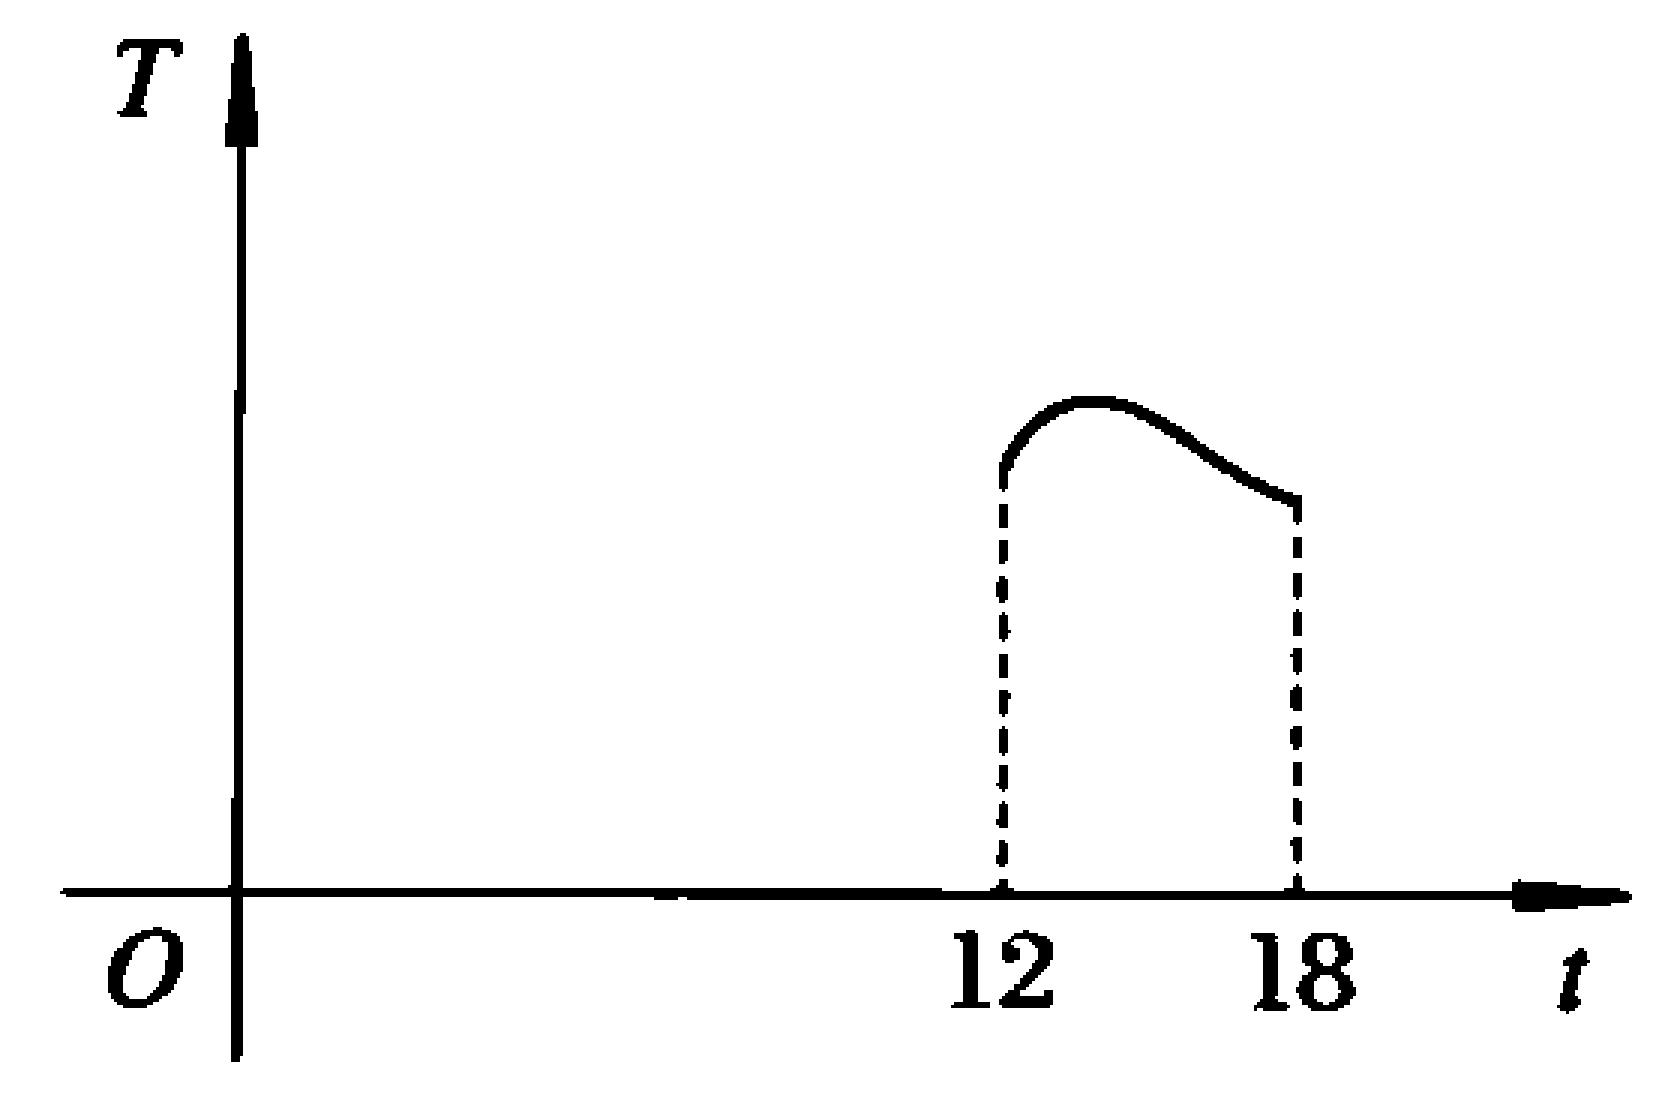
\includegraphics[width=0.35\linewidth]{figures/fig_2_22_1.png}\end{center}
\end{minipage}\par\vfill
\noindent\begin{minipage}{\textwidth}\ProblemHeading{例题}{2.23（改写）}
从甲地到乙地托运行李：不超过50千克时每千克收费0.50元；超过50千克的部分，每千克在0.50元基础上加收0.25元。设行李重 $x$ 千克，求总运费 $f(x)$ 的表达式与定义域。
\end{minipage}\par\vfill
\noindent\begin{minipage}{\textwidth}\ProblemHeading{例题}{2.24（改写）}
设 $f(x)=\sqrt{1-x^2}$、$g(x)=\ln x$，二者均取自然定义域。分别求下列函数的定义域：
\SubQ{1}{$f+g$。}
\SubQ{2}{$f-g$。}
\SubQ{3}{$fg$。}
\end{minipage}\par\vfill
\newpage
\noindent\begin{minipage}{\textwidth}\ProblemHeading{例题}{2.25（改写）}
设 $f(x)=\sqrt{1-x^2}$、$g(x)=\ln x$，二者均取自然定义域。分别求下列函数的定义域：
\SubQ{1}{$f/g$。}
\end{minipage}\par\vfill
\noindent\begin{minipage}{\textwidth}\ProblemHeading{习题}{2.26}
求下列函数的自然定义域：
\SubQ{1}{$f(x)=\sqrt{1-x^2}$。}
\SubQ{2}{$f(x)=\sqrt[3]{\frac{1+x}{1-x}}$。}
\SubQ{3}{$f(x)=\frac{x+1}{x^2+x-2}$。}
\end{minipage}\par\vfill
\noindent\begin{minipage}{\textwidth}\ProblemHeading{习题}{2.27}
求下列函数的自然定义域：
\SubQ{1}{$f(x)=\ln\frac{1+\sin x}{1-\cos x}$。}
\end{minipage}\par\vfill
\newpage
\noindent\begin{minipage}{\textwidth}\ProblemHeading{习题}{2.28}
给定 $f:\mathbb R\to\mathbb R$。若 $f(x)=x$，称 $x$ 为不动点。证明：如果 $f\circ f$ 有唯一不动点，则 $f$ 也有唯一不动点。
\end{minipage}\par\vfill
\noindent\begin{minipage}{\textwidth}\ProblemHeading{习题}{2.29}
设 $f:\mathbb R\to\mathbb R$，$f\circ f$ 恰有两个不动点 $a\ne b$。证明只有两种可能：$f(a)=a$ 且 $f(b)=b$，或 $f(a)=b$ 且 $f(b)=a$。
\end{minipage}\par\vfill
\noindent\begin{minipage}{\textwidth}\ProblemHeading{习题}{2.30}
设 $f:\mathbb R\to\mathbb R$ 且 $f(f(x))=x$ 对每个实数 $x$ 成立。
\SubQ{1}{有多少个满足此条件的函数？}
\SubQ{2}{若再要求 $f$ 在 $\mathbb R$ 上递增，有多少个这样的函数？}
\end{minipage}\par\vfill
\newpage
\noindent\begin{minipage}{\textwidth}\ProblemHeading{习题}{2.31}
求下列函数的 $n$ 次复合 $f^{\circ n}$：
\SubQ{1}{$f(x)=\frac{x}{\sqrt{1+x^2}}$。}
\SubQ{2}{$f(x)=\frac{x}{1+bx}$，在各次复合有定义的点上讨论。}
\end{minipage}\par\vfill
\noindent\begin{minipage}{\textwidth}\ProblemHeading{习题}{2.32}
设 $f:\mathbb R\to\mathbb R$ 满足 $f(x+y)=f(x)+f(y)$。证明对每个有理数 $x$，有 $f(x)=xf(1)$。
\end{minipage}\par\vfill
\noindent\begin{minipage}{\textwidth}\ProblemHeading{习题}{2.33}
若 $f:\mathbb R\to\mathbb R$ 对所有 $x$ 有 $f(x+l)=f(x)$（$l>0$），称 $l$ 为其周期。证明：若每个正数都是 $f$ 的周期，则 $f$ 为常值函数。
\end{minipage}\par\vfill
\newpage
\noindent\begin{minipage}{\textwidth}\ProblemHeading{习题}{2.34}
证明 $f(x)=\sin(x^2)$ 与 $g(x)=\sin x+\cos(\sqrt2x)$ 都不是周期函数。
\end{minipage}\par\vfill
\noindent\begin{minipage}{\textwidth}\ProblemHeading{习题}{2.35}
证明区间 $(-a,a)$ 上的每个函数都能表示为一个奇函数与一个偶函数之和（$a>0$）。
\end{minipage}\par\vfill
\noindent\begin{minipage}{\textwidth}\ProblemHeading{习题}{2.36}
定义双曲余弦 $\cosh x=(\mathrm e^x+\mathrm e^{-x})/2$、双曲正弦 $\sinh x=(\mathrm e^x-\mathrm e^{-x})/2$。证明：
\SubQ{1}{$\cosh x$ 为偶函数，$\sinh x$ 为奇函数。}
\SubQ{2}{$\cosh^2x-\sinh^2x=1$。}
\end{minipage}\par\vfill
\newpage
\noindent\begin{minipage}{\textwidth}\ProblemHeading{习题}{2.37（校订）}
求 $y=\sinh x$（$x\in\mathbb R$）和 $y=\cosh x$（$x\in[0,+\infty)$）的反函数。
\end{minipage}\par\vfill
\noindent\begin{minipage}{\textwidth}\ProblemHeading{习题}{2.38}
设 $T,k>0$ 且 $f(x+T)=kf(x)$ 对每个实数 $x$ 成立。证明存在常数 $a>0$ 与周期为 $T$ 的函数 $\varphi$，使 $f(x)=a^x\varphi(x)$。
\end{minipage}\par\vfill
\noindent\begin{minipage}{\textwidth}\ProblemHeading{习题}{2.39}
设 $a<b$。证明：
\SubQ{1}{若 $f$ 的图像关于直线 $x=a$、$x=b$ 都对称，则 $2(b-a)$ 是 $f$ 的周期。}
\SubQ{2}{若 $f$ 的图像关于直线 $x=a$ 对称，又关于点 $(b,y_0)$ 中心对称，则 $4(b-a)$ 是 $f$ 的周期。}
\SubQ{3}{若 $f$ 的图像关于点 $(a,y_0)$ 和 $(b,y_1)$ 都中心对称，则 $f(x)=\varphi(x)+cx$，其中 $\varphi$ 为周期函数，$c$ 为常数；当 $y_0=y_1$ 时可取 $c=0$。}
\end{minipage}\par\vfill
\newpage
\noindent\begin{minipage}{\textwidth}\ProblemHeading{例题}{2.40}
证明 $\lim_{x\to0}x\sin(1/x)=0$。
\end{minipage}\par\vfill
\noindent\begin{minipage}{\textwidth}\ProblemHeading{例题}{2.41}
求极限 $\lim_{x\to3}(x^2-4x+4)$。
\end{minipage}\par\vfill
\noindent\begin{minipage}{\textwidth}\ProblemHeading{例题}{2.42}
求极限 $\lim_{x\to1}\frac{x^2-1}{x^2-x}$。
\end{minipage}\par\vfill
\newpage
\noindent\begin{minipage}{\textwidth}\ProblemHeading{例题}{2.43}
证明 $\lim_{x\to0}\sin(1/x)$ 不存在。
\end{minipage}\par\vfill
\noindent\begin{minipage}{\textwidth}\ProblemHeading{例题}{2.44}
设 Dirichlet 函数 $D(x)=\begin{cases}1,&x\in\mathbb Q,\\0,&x\notin\mathbb Q.\end{cases}$。证明对每个 $x_0\in\mathbb R$，$\lim_{x\to x_0}D(x)$ 都不存在。
\end{minipage}\par\vfill
\noindent\begin{minipage}{\textwidth}\ProblemHeading{习题}{2.45}
利用函数极限的数列判别法证明夹逼定理：若 $f(x)\le h(x)\le g(x)$ 在 $x_0$ 的某个去心邻域成立，且 $f(x),g(x)\to l$（$x\to x_0$），则 $h(x)\to l$。数列判别法指：函数在 $x_0$ 处极限为 $l$，当且仅当对每个趋于 $x_0$ 且各项不等于 $x_0$ 的数列 $x_n$，都有 $f(x_n)\to l$。
\end{minipage}\par\vfill
\newpage
\noindent\begin{minipage}{\textwidth}\ProblemHeading{例题}{2.46}
证明 $\lim_{x\to0}\frac{\sin x}{x}=1$。
\end{minipage}\par\vfill
\noindent\begin{minipage}{\textwidth}\ProblemHeading{例题}{2.47}
计算极限 $\lim_{x\to0}\frac{1-\cos x}{x^2}$。
\end{minipage}\par\vfill
\noindent\begin{minipage}{\textwidth}\ProblemHeading{例题}{2.48}
定义 Riemann 函数 $R(x)=\begin{cases}1/q,&x=p/q\in\mathbb Q,\ p\in\mathbb Z,\ q\in\mathbb N^*,\ \gcd(|p|,q)=1,\\0,&x\notin\mathbb Q.\end{cases}$（特别地 $R(0)=1$）。证明对任意实数 $x_0$，都有 $\lim_{x\to x_0}R(x)=0$。
\end{minipage}\par\vfill
\newpage
\noindent\begin{minipage}{\textwidth}\ProblemHeading{习题}{2.49}
用 $\varepsilon$--$\delta$ 语言表述 $f(x_0-)=1$。
\end{minipage}\par\vfill
\noindent\begin{minipage}{\textwidth}\ProblemHeading{习题}{2.50}
证明 $\lim_{x\to x_0}f(x)$ 存在且有限，当且仅当 $f(x_0-)=f(x_0+)$ 为有限数。
\end{minipage}\par\vfill
\noindent\begin{minipage}{\textwidth}\ProblemHeading{习题}{2.51}
设 $\lim_{x\to x_0}f(x)=A\in\mathbb R$。用 $\varepsilon$--$\delta$ 语言证明：
\SubQ{1}{$\lim_{x\to x_0}|f(x)|=|A|$。}
\SubQ{2}{$\lim_{x\to x_0}f(x)^2=A^2$。}
\SubQ{3}{若 $A>0$，则 $\lim_{x\to x_0}\sqrt{f(x)}=\sqrt A$。}
\end{minipage}\par\vfill
\newpage
\noindent\begin{minipage}{\textwidth}\ProblemHeading{习题}{2.52}
设 $\lim_{x\to x_0}f(x)=A\in\mathbb R$。用 $\varepsilon$--$\delta$ 语言证明：
\SubQ{1}{$\lim_{x\to x_0}\sqrt[3]{f(x)}=\sqrt[3]A$。}
\end{minipage}\par\vfill
\noindent\begin{minipage}{\textwidth}\ProblemHeading{习题}{2.53}
用 $\varepsilon$--$\delta$ 语言证明：
\SubQ{1}{$\lim_{x\to2}x^3=8$。}
\SubQ{2}{$\lim_{x\to3}\frac{x-3}{x^2-9}=1/6$。}
\SubQ{3}{$\lim_{x\to1}\frac{x^4-1}{x-1}=4$。}
\end{minipage}\par\vfill
\noindent\begin{minipage}{\textwidth}\ProblemHeading{习题}{2.54}
用 $\varepsilon$--$\delta$ 语言证明：
\SubQ{1}{$\lim_{x\to0}\sqrt{1+2x}=1$。}
\SubQ{2}{$\lim_{x\to1^+}\frac{x-1}{\sqrt{x^2-1}}=0$。}
\end{minipage}\par\vfill
\newpage
\noindent\begin{minipage}{\textwidth}\ProblemHeading{习题}{2.55}
设 $f(x)=\begin{cases}x^2,&x\ge2,\\-ax,&x<2.\end{cases}$
\SubQ{1}{求 $f(2+)$ 与 $f(2-)$。}
\SubQ{2}{若 $\lim_{x\to2}f(x)$ 存在，$a$ 应取何值？}
\end{minipage}\par\vfill
\noindent\begin{minipage}{\textwidth}\ProblemHeading{习题}{2.56}
设 $\lim_{x\to x_0}f(x)>a$。证明当 $x$ 充分靠近 $x_0$ 且 $x\ne x_0$ 时，$f(x)>a$。
\end{minipage}\par\vfill
\noindent\begin{minipage}{\textwidth}\ProblemHeading{习题}{2.57}
设 $f(x_0-)<f(x_0+)$。证明存在 $\delta>0$，使得当 $x\in(x_0-\delta,x_0)$、$y\in(x_0,x_0+\delta)$ 时，总有 $f(x)<f(y)$。
\end{minipage}\par\vfill
\newpage
\noindent\begin{minipage}{\textwidth}\ProblemHeading{习题}{2.58}
设 $f$ 在 $(-\infty,x_0)$ 上递增，且存在数列 $x_n<x_0$，使 $x_n\to x_0$、$f(x_n)\to A$。证明 $f(x_0-)=A$。
\end{minipage}\par\vfill
\noindent\begin{minipage}{\textwidth}\ProblemHeading{习题}{2.59}
用精确的肯定语句表述“当 $x\to x_0$ 时，$f(x)$ 不收敛于 $l$”。
\end{minipage}\par\vfill
\noindent\begin{minipage}{\textwidth}\ProblemHeading{习题}{2.60}
设 $A_n\subset[0,1]$ 为有限集且两两不相交，定义\[f(x)=\begin{cases}1/n,&x\in A_n,\\0,&x\in[0,1]\setminus\bigcup_{n\ge1}A_n.\end{cases}\]对任意 $x_0\in[0,1]$，求 $\lim_{x\to x_0}f(x)$（端点取区间内单侧极限）。
\end{minipage}\par\vfill
\newpage
\noindent\begin{minipage}{\textwidth}\ProblemHeading{习题}{2.61}
计算下列极限，其中 $m,n$ 为正整数：
\SubQ{1}{$\lim_{x\to2}\frac{1+x-x^3}{1+x^2}$。}
\SubQ{2}{$\lim_{x\to1}\frac{x^2-2x+1}{x^2-x}$。}
\SubQ{3}{$\lim_{x\to1}\frac{x^m-1}{x-1}$。}
\end{minipage}\par\vfill
\noindent\begin{minipage}{\textwidth}\ProblemHeading{习题}{2.62}
计算下列极限，其中 $m,n$ 为正整数：
\SubQ{1}{$\lim_{x\to1}\frac{x^m-1}{x^n-1}$。}
\SubQ{2}{$\lim_{x\to0}\frac{\sqrt{1+x}-1}{x}$。}
\SubQ{3}{$\lim_{x\to0}\frac{\sqrt{1+x}-\sqrt{1-x}}{x}$。}
\end{minipage}\par\vfill
\noindent\begin{minipage}{\textwidth}\ProblemHeading{习题}{2.63}
计算下列极限，其中 $m,n$ 为正整数：
\SubQ{1}{$\lim_{x\to0}\frac{(1+x)^{1/m}-1}{x}$。}
\SubQ{2}{$\lim_{x\to1}\frac{x+x^2+\cdots+x^m-m}{x-1}$。}
\end{minipage}\par\vfill
\newpage
\noindent\begin{minipage}{\textwidth}\ProblemHeading{习题}{2.64}
求下列极限；出现的 $n$ 为正整数，未参与趋近过程的参数固定：
\SubQ{1}{$\lim_{x\to0}\frac{\sin(ax)}{\sin(bx)}$，其中 $b\ne0$。}
\SubQ{2}{$\lim_{x\to0}\frac{x^2}{1-\cos x}$。}
\SubQ{3}{$\lim_{x\to0}\frac{\sin(\sin x)}x$。}
\end{minipage}\par\vfill
\noindent\begin{minipage}{\textwidth}\ProblemHeading{习题}{2.65}
求下列极限；出现的 $n$ 为正整数，未参与趋近过程的参数固定：
\SubQ{1}{$\lim_{x\to0}\frac{\tan x}x$。}
\SubQ{2}{$\lim_{h\to0}\sin(x+h)$。}
\SubQ{3}{$\lim_{h\to0}\frac{\sin(x+h)-\sin x}h$。}
\end{minipage}\par\vfill
\noindent\begin{minipage}{\textwidth}\ProblemHeading{习题}{2.66}
求下列极限；出现的 $n$ 为正整数，未参与趋近过程的参数固定：
\SubQ{1}{$\lim_{x\to0}\frac{1-\cos x\cos(2x)\cdots\cos(nx)}{x^2}$。}
\SubQ{2}{$\lim_{n\to\infty}\cos(x/2)\cos(x/4)\cdots\cos(x/2^n)$。}
\end{minipage}\par\vfill
\newpage
\noindent\begin{minipage}{\textwidth}\ProblemHeading{习题}{2.67}
求下列极限，其中 $\lfloor x\rfloor$ 为不超过 $x$ 的最大整数：
\SubQ{1}{$\lim_{x\to0}x\lfloor1/x\rfloor$。}
\SubQ{2}{$\lim_{x\to2^+}\frac{\lfloor x\rfloor^2-4}{x^2-4}$。}
\SubQ{3}{$\lim_{x\to2^-}\frac{\lfloor x\rfloor^2+4}{x^2+4}$。}
\end{minipage}\par\vfill
\noindent\begin{minipage}{\textwidth}\ProblemHeading{习题}{2.68}
求下列极限，其中 $\lfloor x\rfloor$ 为不超过 $x$ 的最大整数：
\SubQ{1}{$\lim_{x\to1^-}\frac{\lfloor4x\rfloor}{1+x}$。}
\end{minipage}\par\vfill
\noindent\begin{minipage}{\textwidth}\ProblemHeading{习题}{2.69}
求极限 $\lim_{n\to\infty}n\sin(2\pi n!\,\mathrm e)$。
\end{minipage}\par\vfill
\newpage
\noindent\begin{minipage}{\textwidth}\ProblemHeading{习题}{2.70}
设 $f(x)=1$（$x\ne0$），$f(0)=0$；$g(t)=1/q$ 当 $t=p/q$ 是既约有理数且 $q>0$，$g(t)=0$ 当 $t$ 为无理数。虽然 $\lim_{x\to0}f(x)=1$、$\lim_{t\to0}g(t)=0$，复合函数 $f(g(t))$ 却在 $t=0$ 处没有极限。说明为何不能在这里应用复合函数极限定理。
\end{minipage}\par\vfill
\noindent\begin{minipage}{\textwidth}\ProblemHeading{习题}{2.71}
定义 $f(x)=q$，当 $x=p/q$ 为既约有理数且 $q>0$；对无理数令 $f(x)=0$（因此 $f(0)=1$）。证明 $f$ 在实轴上每一点的任意邻域内都无界。
\end{minipage}\par\vfill
\noindent\begin{minipage}{\textwidth}\ProblemHeading{习题}{2.72}
用精确的量词语言给出 $\lim_{x\to+\infty}f(x)=l$（$l\in\mathbb R$）的定义。
\end{minipage}\par\vfill
\newpage
\noindent\begin{minipage}{\textwidth}\ProblemHeading{例题}{2.73}
设 $f(x)=(1+1/\lfloor x\rfloor)^{\lfloor x\rfloor}$（$x\ge1$），其中 $\lfloor x\rfloor$ 为不超过 $x$ 的最大整数。求 $\lim_{x\to+\infty}f(x)$。
\end{minipage}\par\vfill
\noindent\begin{minipage}{\textwidth}\ProblemHeading{习题}{2.74}
用 $\varepsilon$--$A$ 语言证明 $\lim_{x\to+\infty}(1+1/\lfloor x\rfloor)=1$，其中 $\lfloor x\rfloor$ 表示取整。
\end{minipage}\par\vfill
\noindent\begin{minipage}{\textwidth}\ProblemHeading{例题}{2.75（改写）}
证明 $\lim_{x\to\infty}(1+1/x)^x=\mathrm e$，这里 $x\to\infty$ 表示 $|x|\to+\infty$，需同时考虑正、负两个方向。
\end{minipage}\par\vfill
\newpage
\noindent\begin{minipage}{\textwidth}\ProblemHeading{习题}{2.76}
用 $\varepsilon$--$A$ 语言证明：
\SubQ{1}{$\lim_{x\to-\infty}\frac{x^2+1}{3x^2-x+1}=1/3$。}
\SubQ{2}{$\lim_{x\to\infty}\frac{3x+2}{2x+3}=3/2$。}
\SubQ{3}{$\lim_{x\to+\infty}(x-\sqrt{x^2-a})=0$，其中 $a$ 固定。}
\end{minipage}\par\vfill
\noindent\begin{minipage}{\textwidth}\ProblemHeading{习题}{2.77}
用 $\varepsilon$--$A$ 语言证明：
\SubQ{1}{$\lim_{x\to+\infty}(\sqrt{x+1}-\sqrt{x-1})=0$。}
\end{minipage}\par\vfill
\noindent\begin{minipage}{\textwidth}\ProblemHeading{习题}{2.78}
分别求常数 $a,b$，使下列极限成立：
\SubQ{1}{$\lim_{x\to\infty}\left(\frac{x^2+1}{x+1}-ax-b\right)=0$。}
\SubQ{2}{$\lim_{x\to+\infty}(\sqrt{x^2-x+1}-ax-b)=0$。}
\SubQ{3}{$\lim_{x\to-\infty}(\sqrt{x^2-x+1}-ax-b)=0$。}
\end{minipage}\par\vfill
\newpage
\noindent\begin{minipage}{\textwidth}\ProblemHeading{习题}{2.79}
证明 $\lim_{x\to+\infty}(\sin\sqrt{x+1}-\sin\sqrt{x-1})=0$。
\end{minipage}\par\vfill
\noindent\begin{minipage}{\textwidth}\ProblemHeading{习题}{2.80}
设常数 $a_1,\ldots,a_n$ 满足 $a_1+\cdots+a_n=0$。证明 $\lim_{x\to+\infty}\sum_{k=1}^n a_k\sin\sqrt{x+k}=0$。
\end{minipage}\par\vfill
\noindent\begin{minipage}{\textwidth}\ProblemHeading{习题}{2.81}
求极限 $\lim_{n\to\infty}\sin(\pi\sqrt{n^2+1})$。
\end{minipage}\par\vfill
\newpage
\noindent\begin{minipage}{\textwidth}\ProblemHeading{习题}{2.82}
求下列极限，其中 $a,x$ 在其未参与趋近过程时均为固定实参数：
\SubQ{1}{$\lim_{x\to\infty}\left(\frac{1+x}{3+x}\right)^x$。}
\SubQ{2}{$\lim_{x\to\infty}\left(\frac{x+a}{x-a}\right)^x$。}
\SubQ{3}{$\lim_{x\to0}(1-2x)^{1/x}$。}
\end{minipage}\par\vfill
\noindent\begin{minipage}{\textwidth}\ProblemHeading{习题}{2.83}
求下列极限，其中 $a,x$ 在其未参与趋近过程时均为固定实参数：
\SubQ{1}{$\lim_{n\to\infty}\left(\frac{n+x}{n-2}\right)^n$。}
\end{minipage}\par\vfill
\noindent\begin{minipage}{\textwidth}\ProblemHeading{习题}{2.84}
设 $f(x)=\lim_{n\to\infty}n^x\bigl[(1+1/n)^{n+1}-(1+1/n)^n\bigr]$。求该极限为有限实数时的自然定义域及 $f(x)$ 的表达式。
\end{minipage}\par\vfill
\newpage
\noindent\begin{minipage}{\textwidth}\ProblemHeading{习题}{2.85}
设常数 $a_1,\ldots,a_n$ 满足：对任意 $x\in(-1,1)$，都有 $\left|\sum_{k=1}^n a_k\sin(kx)\right|\le|\sin x|$。证明 $\left|\sum_{k=1}^n ka_k\right|\le1$。
\end{minipage}\par\vfill
\noindent\begin{minipage}{\textwidth}\ProblemHeading{习题}{2.86}
证明函数在正无穷处具有有限极限的 Cauchy 准则：$\lim_{x\to+\infty}f(x)$ 存在且有限，当且仅当对任意 $\varepsilon>0$，存在 $A>0$，使任意 $x_1,x_2>A$ 都满足 $|f(x_1)-f(x_2)|<\varepsilon$。
\end{minipage}\par\vfill
\noindent\begin{minipage}{\textwidth}\ProblemHeading{习题}{2.87}
设 $f:\mathbb R\to\mathbb R$ 为周期函数且 $\lim_{x\to+\infty}f(x)=0$。证明 $f\equiv0$。
\end{minipage}\par\vfill
\newpage
\noindent\begin{minipage}{\textwidth}\ProblemHeading{习题}{2.88}
设 $f:(0,+\infty)\to\mathbb R$ 满足 $f(2x)=f(x)$，且 $\lim_{x\to+\infty}f(x)$ 存在且有限。证明 $f$ 为常数。
\end{minipage}\par\vfill
\noindent\begin{minipage}{\textwidth}\ProblemHeading{习题}{2.89}
设 $a,b>1$，函数 $f:\mathbb R\to\mathbb R$ 在原点的某个邻域内有界，且对每个实数 $x$ 满足 $f(ax)=bf(x)$。证明 $\lim_{x\to0}f(x)=f(0)$。
\end{minipage}\par\vfill
\noindent\begin{minipage}{\textwidth}\ProblemHeading{习题}{2.90}
设 $f,g:\mathbb R\to\mathbb R$ 都是周期函数，且 $\lim_{x\to+\infty}[f(x)-g(x)]=0$。证明 $f=g$。
\end{minipage}\par\vfill
\newpage
\noindent\begin{minipage}{\textwidth}\ProblemHeading{习题}{2.91}
设数列 $x_n>0$。
\SubQ{1}{证明 $\varlimsup_{n\to\infty}\left(\frac{x_1+x_{n+1}}{x_n}\right)^n\ge\mathrm e$。}
\SubQ{2}{证明上述不等式中的常数 $\mathrm e$ 不能提高。}
\end{minipage}\par\vfill
\noindent\begin{minipage}{\textwidth}\ProblemHeading{习题}{2.92}
求下列无穷小或无穷大的阶，并说明所用的标准比较量；当双侧与单侧结论不同时，分别讨论。出现的 $n$ 为正整数。
\SubQ{1}{$x-5x^3+x^{10}$，$x\to0$。}
\SubQ{2}{$x-5x^3+x^{10}$，$x\to\infty$。}
\SubQ{3}{$\dfrac{x+1}{x^4+1}$，$x\to\infty$。}
\end{minipage}\par\vfill
\noindent\begin{minipage}{\textwidth}\ProblemHeading{习题}{2.93}
求下列无穷小或无穷大的阶，并说明所用的标准比较量；当双侧与单侧结论不同时，分别讨论。出现的 $n$ 为正整数。
\SubQ{1}{$x^3-3x+2$，$x\to1$。}
\SubQ{2}{$\dfrac{2x^5}{x^3-3x+1}$，$x\to+\infty$。}
\SubQ{3}{$\dfrac1{\sin(\pi x)}$，$x\to1$。}
\end{minipage}\par\vfill
\newpage
\noindent\begin{minipage}{\textwidth}\ProblemHeading{习题}{2.94}
求下列无穷小或无穷大的阶，并说明所用的标准比较量；当双侧与单侧结论不同时，分别讨论。出现的 $n$ 为正整数。
\SubQ{1}{$\sqrt{x\sin x}$，$x\to0$。}
\SubQ{2}{$\sqrt{x^2+\sqrt[3]x}$，$x\to0^+$（从自然定义域趋近）。}
\SubQ{3}{$\sqrt{x^2+\sqrt[3]x}$，$x\to\infty$。}
\end{minipage}\par\vfill
\noindent\begin{minipage}{\textwidth}\ProblemHeading{习题}{2.95}
求下列无穷小或无穷大的阶，并说明所用的标准比较量；当双侧与单侧结论不同时，分别讨论。出现的 $n$ 为正整数。
\SubQ{1}{$\sqrt{1+x}-\sqrt{1-x}$，$x\to0$。}
\SubQ{2}{$\sin\bigl(\sqrt{1+\sqrt{1+\sqrt x}}-\sqrt2\bigr)$，$x\to0^+$。}
\SubQ{3}{$\sqrt{1+\tan x}-\sqrt{1-\sin x}$，$x\to0$。}
\end{minipage}\par\vfill
\noindent\begin{minipage}{\textwidth}\ProblemHeading{习题}{2.96}
求下列无穷小或无穷大的阶，并说明所用的标准比较量；当双侧与单侧结论不同时，分别讨论。出现的 $n$ 为正整数。
\SubQ{1}{$\sqrt{x+\sqrt{x+\sqrt x}}$，$x\to+\infty$。}
\SubQ{2}{$(1+x)(1+x^2)\cdots(1+x^n)$，$x\to+\infty$。}
\end{minipage}\par\vfill
\newpage
\noindent\begin{minipage}{\textwidth}\ProblemHeading{习题}{2.97（校订）}
设 $\alpha(x)$ 在 $x_0$ 的某个去心邻域内不为零，且 $\alpha(x)=o(1)$（$x\to x_0$）。证明下列小 $o$ 运算规则；各处 $o(\alpha)$ 可代表不同函数：
\SubQ{1}{$o(\alpha)+o(\alpha)=o(\alpha)$。}
\SubQ{2}{$o(c\alpha)=o(\alpha)$，其中 $c$ 为非零常数。}
\SubQ{3}{$[o(\alpha)]^k=o(\alpha^k)$，其中 $k$ 为正整数。}
\end{minipage}\par\vfill
\noindent\begin{minipage}{\textwidth}\ProblemHeading{习题}{2.98（校订）}
设 $\alpha(x)$ 在 $x_0$ 的某个去心邻域内不为零，且 $\alpha(x)=o(1)$（$x\to x_0$）。证明下列小 $o$ 运算规则；各处 $o(\alpha)$ 可代表不同函数：
\SubQ{1}{$\dfrac1{1+\alpha}=1-\alpha+o(\alpha)$。}
\end{minipage}\par\vfill
\noindent\begin{minipage}{\textwidth}\ProblemHeading{习题}{2.99}
利用等价无穷小求下列极限，其中 $n$ 为正整数：
\SubQ{1}{$\lim_{x\to0}\dfrac{x\tan^4x}{\sin^3x(1-\cos x)}$。}
\SubQ{2}{$\lim_{x\to0}\dfrac{\sqrt{1+x^2}-1}{1-\cos x}$。}
\SubQ{3}{$\lim_{x\to0}\dfrac{\sqrt{1+x^4}-1}{1-\cos^2x}$。}
\end{minipage}\par\vfill
\newpage
\noindent\begin{minipage}{\textwidth}\ProblemHeading{习题}{2.100}
利用等价无穷小求下列极限，其中 $n$ 为正整数：
\SubQ{1}{$\lim_{x\to0}\dfrac{\tan(\tan x)}{\sin x}$。}
\SubQ{2}{$\lim_{x\to0}\dfrac{(1+x+x^2)^{1/n}-1}{\sin(2x)}$。}
\end{minipage}\par\vfill
\noindent\begin{minipage}{\textwidth}\ProblemHeading{习题}{2.101}
设 $\lim_{x\to0}f(x)=0$，且 $f(x)-f(x/2)=o(x)$（$x\to0$）。证明 $f(x)=o(x)$。
\end{minipage}\par\vfill
\noindent\begin{minipage}{\textwidth}\ProblemHeading{习题}{2.102}
设可列个函数 $f_n:(0,+\infty)\to\mathbb R$ 在 $x\to+\infty$ 时均为无穷大。证明存在函数 $f:(0,+\infty)\to\mathbb R$，其无穷大阶数高于每个 $f_n$，即 $|f(x)|\to+\infty$ 且对每个固定 $n$ 有 $f_n(x)/f(x)\to0$。
\end{minipage}\par\vfill
\newpage
\noindent\begin{minipage}{\textwidth}\ProblemHeading{例题}{2.103（改写）}
用连续性的定义证明常值函数 $f(x)=c$（$c\in\mathbb R$）在实轴上处处连续。
\end{minipage}\par\vfill
\noindent\begin{minipage}{\textwidth}\ProblemHeading{例题}{2.104（改写）}
用连续性的定义证明函数 $f(x)=x$ 在实轴上处处连续。
\end{minipage}\par\vfill
\noindent\begin{minipage}{\textwidth}\ProblemHeading{例题}{2.105（改写）}
证明正弦函数与余弦函数在每个实数点都连续。
\end{minipage}\par\vfill
\newpage
\noindent\begin{minipage}{\textwidth}\ProblemHeading{例题}{2.106}
设 Dirichlet 函数 $D(x)=\begin{cases}1,&x\in\mathbb Q,\\0,&x\notin\mathbb Q.\end{cases}$。证明：
\SubQ{1}{$D$ 在每一点都不连续。}
\SubQ{2}{函数 $f(x)=xD(x)$ 仅在 $x=0$ 处连续。}
\end{minipage}\par\vfill
\noindent\begin{minipage}{\textwidth}\ProblemHeading{例题}{2.107（改写）}
证明指数函数 $f(x)=a^x$（$a>0$，$a\ne1$）在实轴上处处连续。
\end{minipage}\par\vfill
\noindent\begin{minipage}{\textwidth}\ProblemHeading{习题}{2.108}
回答下列问题：
\SubQ{1}{设 $f(x)=\sin(1/x)$（$x\ne0$）。能否定义 $f(0)$，使其在 $x=0$ 处连续？}
\SubQ{2}{设 $f(x)=x\sin(1/x)$。如何理解该表达式的自然定义域？若要连续地扩充至 $x=0$，应怎样定义 $f(0)$？}
\SubQ{3}{设 $f$ 在 $x_0$ 的邻域有定义且 $\lim_{h\to0}f(x_0+h)=f(x_0)$。$f$ 是否在 $x_0$ 处连续？}
\end{minipage}\par\vfill
\newpage
\noindent\begin{minipage}{\textwidth}\ProblemHeading{习题}{2.109}
回答下列问题：
\SubQ{1}{设 $f$ 在 $x_0$ 的邻域有定义且 $\lim_{h\to0}[f(x_0+h)-f(x_0-h)]=0$。$f$ 是否在 $x_0$ 处连续？}
\SubQ{2}{设连续函数 $f$ 在区间 $(a,b)$ 内的所有有理点上取零值。$f$ 是怎样的函数？}
\end{minipage}\par\vfill
\noindent\begin{minipage}{\textwidth}\ProblemHeading{习题}{2.110}
研究下列函数在 $x=0$ 处的连续性，其中 $\lfloor x\rfloor$ 表示取整：
\SubQ{1}{$f(x)=|x|$。}
\SubQ{2}{$f(x)=\lfloor x\rfloor$。}
\SubQ{3}{$f(x)=\begin{cases}\mathrm e^{-1/x^2},&x\ne0,\\0,&x=0.\end{cases}$}
\end{minipage}\par\vfill
\noindent\begin{minipage}{\textwidth}\ProblemHeading{习题}{2.111}
研究下列函数在 $x=0$ 处的连续性，其中 $\lfloor x\rfloor$ 表示取整：
\SubQ{1}{$f(x)=\begin{cases}\sin x/|x|,&x\ne0,\\1,&x=0.\end{cases}$}
\SubQ{2}{$f(x)=\begin{cases}(1+x^2)^{1/x^2},&x\ne0,\\2.7,&x=0.\end{cases}$}
\end{minipage}\par\vfill
\newpage
\noindent\begin{minipage}{\textwidth}\ProblemHeading{习题}{2.112}
确定常数 $a,b,c$，使函数\[f(x)=\begin{cases}-1,&x\le-1,\\ax^2+bx+c,&|x|<1\text{ 且 }x\ne0,\\0,&x=0,\\1,&x\ge1\end{cases}\]在整个实轴上连续。
\end{minipage}\par\vfill
\noindent\begin{minipage}{\textwidth}\ProblemHeading{习题}{2.113}
分别讨论下列情况下 $f+g$ 和 $fg$ 在 $x_0$ 处的连续性：
\SubQ{1}{$f$ 在 $x_0$ 处连续，而 $g$ 在 $x_0$ 处不连续。}
\SubQ{2}{$f,g$ 在 $x_0$ 处都不连续。}
\end{minipage}\par\vfill
\noindent\begin{minipage}{\textwidth}\ProblemHeading{习题}{2.114}
设 $f$ 在 $x_0$ 处连续且 $f(x_0)>0$。证明当 $x$ 充分靠近 $x_0$ 时，$f(x)>f(x_0)/2$。
\end{minipage}\par\vfill
\newpage
\noindent\begin{minipage}{\textwidth}\ProblemHeading{习题}{2.115}
设 $f$ 在 $x_0$ 处连续。证明 $|f|$ 与 $f^2$ 都在 $x_0$ 处连续；反之是否成立？
\end{minipage}\par\vfill
\noindent\begin{minipage}{\textwidth}\ProblemHeading{习题}{2.116}
设 $f,g$ 在 $(a,b)$ 上连续，令 $F(x)=\max\{f(x),g(x)\}$、$G(x)=\min\{f(x),g(x)\}$。证明 $F,G$ 在 $(a,b)$ 上连续。
\end{minipage}\par\vfill
\noindent\begin{minipage}{\textwidth}\ProblemHeading{习题}{2.117}
设 $f$ 的间断点全为可去间断点，令 $g(x)=\lim_{t\to x}f(t)$。证明 $g$ 是连续函数。
\end{minipage}\par\vfill
\newpage
\noindent\begin{minipage}{\textwidth}\ProblemHeading{习题}{2.118}
设 $f$ 在 $\mathbb R$ 上递增或递减，定义 $F(x)=f(x+)$。证明 $F$ 在 $\mathbb R$ 上右连续。
\end{minipage}\par\vfill
\noindent\begin{minipage}{\textwidth}\ProblemHeading{习题}{2.119}
设 $f$ 在 $\mathbb R$ 上连续，且对任意实数 $x,y$ 有 $f(x+y)=f(x)+f(y)$。证明 $f(x)=f(1)x$ 对所有实数 $x$ 成立。
\end{minipage}\par\vfill
\noindent\begin{minipage}{\textwidth}\ProblemHeading{习题}{2.120}
设 $f_1,f_2,f_3\in C[a,b]$，定义 $f(x)$ 为三个数 $f_1(x),f_2(x),f_3(x)$ 的中位数。证明 $f\in C[a,b]$。
\end{minipage}\par\vfill
\newpage
\noindent\begin{minipage}{\textwidth}\ProblemHeading{习题}{2.121}
设 $f$ 在 $(a,b)$ 内的间断点均为第一类间断点，且对任意 $x,y\in(a,b)$ 有\[f\left(\frac{x+y}2\right)\le\frac{f(x)+f(y)}2.\]证明 $f\in C(a,b)$。
\end{minipage}\par\vfill
\noindent\begin{minipage}{\textwidth}\ProblemHeading{习题}{2.122}
设 $f:\mathbb R\to\mathbb R$ 满足 $f(x+y)=f(x)+f(y)$。证明：
\SubQ{1}{若 $f$ 在某一点 $x_0$ 连续，则 $f(x)=f(1)x$。}
\SubQ{2}{若 $f$ 在 $\mathbb R$ 上单调，则 $f(x)=f(1)x$。}
\end{minipage}\par\vfill
\noindent\begin{minipage}{\textwidth}\ProblemHeading{习题}{2.123}
设 $f$ 是 $\mathbb R$ 上不恒为零的连续函数，且 $f(x+y)=f(x)f(y)$ 对任意实数 $x,y$ 成立。证明 $f(x)=a^x$，其中 $a=f(1)>0$。
\end{minipage}\par\vfill
\newpage
\noindent\begin{minipage}{\textwidth}\ProblemHeading{习题}{2.124（校订）}
设 $f\in C(0,+\infty)$，且对任意 $x,y>0$ 有 $f(xy)=f(x)f(y)$。证明 $f\equiv0$，或存在实常数 $a$ 使 $f(x)=x^a$。
\end{minipage}\par\vfill
\noindent\begin{minipage}{\textwidth}\ProblemHeading{习题}{2.125}
设 $n\in\mathbb N^*$。求满足函数方程 $f(x+y^n)=f(x)+[f(y)]^n$（$x,y\in\mathbb R$）的所有连续实函数 $f$。
\end{minipage}\par\vfill
\noindent\begin{minipage}{\textwidth}\ProblemHeading{习题}{2.126}
设 $f:\mathbb R\to\mathbb R$ 满足 $f(x^2)=f(x)$，且 $f$ 在 $x=0$ 与 $x=1$ 处连续。证明 $f$ 为常值函数。
\end{minipage}\par\vfill
\newpage
\noindent\begin{minipage}{\textwidth}\ProblemHeading{例题}{2.127}
计算下列极限：
\SubQ{1}{$\lim_{x\to0}\dfrac{\ln(1+x)}x$。}
\SubQ{2}{$\lim_{x\to0}\dfrac{a^x-1}x$，其中 $a>0$。}
\SubQ{3}{$\lim_{x\to0}\dfrac{(1+x)^\alpha-1}x$，其中 $\alpha\in\mathbb R$。}
\end{minipage}\par\vfill
\noindent\begin{minipage}{\textwidth}\ProblemHeading{例题}{2.128}
设 $m,n$ 为正整数。计算极限 $\lim_{x\to1}\left(\dfrac m{x^m-1}-\dfrac n{x^n-1}\right)$。
\end{minipage}\par\vfill
\noindent\begin{minipage}{\textwidth}\ProblemHeading{例题}{2.129}
设 $a_1,\ldots,a_n$ 为给定正数。计算极限 $\lim_{x\to0}\left(\dfrac{a_1^x+\cdots+a_n^x}{n}\right)^{1/x}$。
\end{minipage}\par\vfill
\newpage
\noindent\begin{minipage}{\textwidth}\ProblemHeading{例题}{2.130}
计算极限 $\lim_{x\to\infty}(\cos(1/x))^{x^2}$。
\end{minipage}\par\vfill
\noindent\begin{minipage}{\textwidth}\ProblemHeading{习题}{2.131}
计算下列极限，其中 $n$ 为正整数、$a$ 为固定实数：
\SubQ{1}{$\lim_{x\to1}\dfrac{x^2-1}{2x^2-x-1}$。}
\SubQ{2}{$\lim_{x\to0}\dfrac{(1+x)^5-(1+5x)}{x^2+x^5}$。}
\SubQ{3}{$\lim_{x\to0}\dfrac{(1+x)(1+2x)(1+3x)-1}x$。}
\end{minipage}\par\vfill
\noindent\begin{minipage}{\textwidth}\ProblemHeading{习题}{2.132}
计算下列极限，其中 $n$ 为正整数、$a$ 为固定实数：
\SubQ{1}{$\lim_{x\to a}\dfrac{x^n-a^n-na^{n-1}(x-a)}{(x-a)^2}$。}
\SubQ{2}{$\lim_{x\to1}\dfrac{x^{n+1}-(n+1)x+n}{(x-1)^2}$。}
\end{minipage}\par\vfill
\newpage
\noindent\begin{minipage}{\textwidth}\ProblemHeading{习题}{2.133}
计算下列极限，其中 $m,n$ 为正整数，$\alpha,\beta$ 为实常数（最后一式取 $n\ge2$）：
\SubQ{1}{$\lim_{x\to1}\dfrac{\sqrt[m]x-1}{\sqrt[n]x-1}$。}
\SubQ{2}{$\lim_{x\to0}\dfrac{\sqrt[m]{1+\alpha x}-1}x$。}
\SubQ{3}{$\lim_{x\to0}\dfrac{\sqrt[m]{1+\alpha x}-\sqrt[n]{1+\beta x}}x$。}
\end{minipage}\par\vfill
\noindent\begin{minipage}{\textwidth}\ProblemHeading{习题}{2.134}
计算下列极限，其中 $m,n$ 为正整数，$\alpha,\beta$ 为实常数（最后一式取 $n\ge2$）：
\SubQ{1}{$\lim_{x\to1}\dfrac{(1-\sqrt x)(1-\sqrt[3]x)\cdots(1-\sqrt[n]x)}{(1-x)^{n-1}}$。}
\end{minipage}\par\vfill
\noindent\begin{minipage}{\textwidth}\ProblemHeading{习题}{2.135（校订）}
计算下列极限：
\SubQ{1}{$\lim_{x\to0}\left(\dfrac{1+\tan x}{1+\sin x}\right)^{1/\sin x}$。}
\SubQ{2}{$\lim_{x\to0}\left(\dfrac{\cos x}{\cos(2x)}\right)^{1/x^2}$。}
\SubQ{3}{$\lim_{x\to\pi/4}(\tan x)^{\tan(2x)}$。}
\end{minipage}\par\vfill
\newpage
\noindent\begin{minipage}{\textwidth}\ProblemHeading{习题}{2.136（校订）}
计算下列极限：
\SubQ{1}{$\lim_{x\to\pi/2}(\sin x)^{\tan x}$。}
\SubQ{2}{$\lim_{x\to+\infty}(\sin(1/x)+\cos(1/x))^x$。}
\SubQ{3}{$\lim_{x\to0^+}(\cos\sqrt x)^{1/x}$。}
\end{minipage}\par\vfill
\noindent\begin{minipage}{\textwidth}\ProblemHeading{习题}{2.137（校订）}
计算下列极限：
\SubQ{1}{$\lim_{n\to\infty}\cos^n(x/\sqrt n)$，其中 $x\in\mathbb R$ 固定。}
\SubQ{2}{$\lim_{x\to0}(2\mathrm e^{x/(1+x)}-1)^{(x^2+1)/x}$。}
\SubQ{3}{$\lim_{x\to a}\left(\dfrac{\sin x}{\sin a}\right)^{1/(x-a)}$，其中 $a\notin\pi\mathbb Z$。}
\end{minipage}\par\vfill
\noindent\begin{minipage}{\textwidth}\ProblemHeading{习题}{2.138}
设 $|x|<1$，求极限 $\lim_{n\to\infty}\left(1+\dfrac{x+x^2+\cdots+x^n}n\right)^n$。
\end{minipage}\par\vfill
\newpage
\noindent\begin{minipage}{\textwidth}\ProblemHeading{例题}{2.139}
证明函数 $f(x)=\sqrt x$ 在 $[0,+\infty)$ 上一致连续。
\end{minipage}\par\vfill
\noindent\begin{minipage}{\textwidth}\ProblemHeading{例题}{2.140（改写）}
证明函数 $\sin x$ 与 $\cos x$ 在 $\mathbb R$ 上一致连续。
\end{minipage}\par\vfill
\noindent\begin{minipage}{\textwidth}\ProblemHeading{例题}{2.141}
在区间 $I=[0,+\infty)$ 上，证明：
\SubQ{1}{函数 $f(x)=x$ 一致连续。}
\SubQ{2}{当整数 $n\ge2$ 时，函数 $f(x)=x^n$ 不一致连续。}
\end{minipage}\par\vfill
\newpage
\noindent\begin{minipage}{\textwidth}\ProblemHeading{例题}{2.142}
证明函数 $f(x)=\sin(1/x)$ 在 $(0,1)$ 上不一致连续。
\end{minipage}\par\vfill
\noindent\begin{minipage}{\textwidth}\ProblemHeading{例题}{2.143（改写）}
设 $\sigma>0$。证明函数 $f(x)=1/x$ 在 $[\sigma,+\infty)$ 上一致连续。
\end{minipage}\par\vfill
\noindent\begin{minipage}{\textwidth}\ProblemHeading{习题}{2.144}
研究下列函数在指定定义域上的一致连续性：
\SubQ{1}{$f(x)=\cos(1/x)$，$x>0$。}
\SubQ{2}{$f(x)=\sin^2x$，$x\in\mathbb R$。}
\SubQ{3}{$f(x)=\sqrt[3]x$，$x\ge0$。}
\end{minipage}\par\vfill
\newpage
\noindent\begin{minipage}{\textwidth}\ProblemHeading{习题}{2.145}
研究下列函数在指定定义域上的一致连续性：
\SubQ{1}{$f(x)=\sin(x^2)$，$x\in\mathbb R$。}
\SubQ{2}{$f(x)=\dfrac{x}{1+x^2\sin^2x}$，$x\ge0$。}
\end{minipage}\par\vfill
\noindent\begin{minipage}{\textwidth}\ProblemHeading{习题}{2.146}
设函数 $f,g$ 在区间 $I$ 上一致连续。证明 $f+g$ 在 $I$ 上一致连续。
\end{minipage}\par\vfill
\noindent\begin{minipage}{\textwidth}\ProblemHeading{习题}{2.147}
设 $a<b$ 为有限实数，$f$ 在 $(a,b)$ 上一致连续。证明 $f(a+)$ 与 $f(b-)$ 存在且有限。
\end{minipage}\par\vfill
\newpage
\noindent\begin{minipage}{\textwidth}\ProblemHeading{习题}{2.148}
设 $f$ 在 $[0,+\infty)$ 上一致连续，且对每个 $x\in[0,1]$ 有 $\lim_{n\to\infty}f(x+n)=0$。证明 $\lim_{x\to+\infty}f(x)=0$。再举例说明：若只假设 $f$ 在 $[0,+\infty)$ 上连续，则上述结论未必成立。
\end{minipage}\par\vfill
\noindent\begin{minipage}{\textwidth}\ProblemHeading{习题}{2.149}
设 $a>0$，函数 $f$ 在 $[a,+\infty)$ 上满足 Lipschitz 条件：存在常数 $k>0$，使任意 $x,y\ge a$ 都有 $|f(x)-f(y)|\le k|x-y|$。证明函数 $f(x)/x$ 在 $[a,+\infty)$ 上一致连续。
\end{minipage}\par\vfill
\noindent\begin{minipage}{\textwidth}\ProblemHeading{习题}{2.150}
举例说明：函数在无穷区间 $[a,+\infty)$ 上连续，并不能保证它在该区间上有界。
\end{minipage}\par\vfill
\newpage
\noindent\begin{minipage}{\textwidth}\ProblemHeading{例题}{2.151}
证明方程 $2^x-4x=0$ 在区间 $(0,1/2)$ 内至少有一个根。
\end{minipage}\par\vfill
\noindent\begin{minipage}{\textwidth}\ProblemHeading{例题}{2.152}
证明任意实系数奇次代数方程都至少有一个实根。
\end{minipage}\par\vfill
\noindent\begin{minipage}{\textwidth}\ProblemHeading{例题}{2.153}
某短跑运动员用10秒跑完100米。将其沿跑道前进的路程视为时间的连续函数，证明至少存在连续的1秒时间段，他在这段时间内恰好前进10米。
\end{minipage}\par\vfill
\newpage
\noindent\begin{minipage}{\textwidth}\ProblemHeading{习题}{2.154}
设 $a<b$ 为有限实数，$f$ 在 $(a,b)$ 上一致连续。证明 $f$ 在 $(a,b)$ 上有界。
\end{minipage}\par\vfill
\noindent\begin{minipage}{\textwidth}\ProblemHeading{习题}{2.155}
设 $f,g$ 都在区间 $I$ 上一致连续。乘积 $fg$ 是否在 $I$ 上一致连续？分别讨论 $I$ 为有限区间与无穷区间的情形。
\end{minipage}\par\vfill
\noindent\begin{minipage}{\textwidth}\ProblemHeading{习题}{2.156}
设 $f$ 在有限开区间 $(a,b)$ 上连续，且 $f(a+),f(b-)$ 存在且有限。证明 $f$ 在 $(a,b)$ 上一致连续。
\end{minipage}\par\vfill
\newpage
\noindent\begin{minipage}{\textwidth}\ProblemHeading{习题}{2.157}
设 $f$ 在 $[a,+\infty)$ 上连续，且 $f(+\infty)$ 存在且有限。证明 $f$ 在 $[a,+\infty)$ 上一致连续。
\end{minipage}\par\vfill
\noindent\begin{minipage}{\textwidth}\ProblemHeading{习题}{2.158}
设 $f$ 在 $[a,+\infty)$ 上连续，存在常数 $b,c$ 使 $\lim_{x\to+\infty}[f(x)-bx-c]=0$。证明 $f$ 在 $[a,+\infty)$ 上一致连续。
\end{minipage}\par\vfill
\noindent\begin{minipage}{\textwidth}\ProblemHeading{习题}{2.159}
证明三次方程 $x^3+2x-1=0$ 有唯一实根，且此根位于 $(0,1)$ 内。
\end{minipage}\par\vfill
\newpage
\noindent\begin{minipage}{\textwidth}\ProblemHeading{习题}{2.160}
设 $n$ 为正整数，$\varphi\in C(\mathbb R)$，且 $\lim_{x\to+\infty}\varphi(x)/x^n=\lim_{x\to-\infty}\varphi(x)/x^n=0$。证明：
\SubQ{1}{当 $n$ 为奇数时，方程 $x^n+\varphi(x)=0$ 至少有一个实根。}
\SubQ{2}{当 $n$ 为偶数时，存在 $y\in\mathbb R$，使任意实数 $x$ 都满足 $y^n+\varphi(y)\le x^n+\varphi(x)$。}
\end{minipage}\par\vfill
\noindent\begin{minipage}{\textwidth}\ProblemHeading{习题}{2.161（校订）}
设 $f\in C[0,1]$ 且 $f(0)=f(1)$。证明对每个正整数 $n$，存在 $x_n\in[0,1-1/n]$，使 $f(x_n)=f(x_n+1/n)$。
\end{minipage}\par\vfill
\noindent\begin{minipage}{\textwidth}\ProblemHeading{习题}{2.162}
设 $f\in C(\mathbb R)$ 且 $\lim_{x\to\pm\infty}f(x)=+\infty$。假设 $f$ 在点 $a$ 取得最小值，且 $f(a)<a$。证明复合函数 $f\circ f$ 至少在两个不同的点取得最小值。
\end{minipage}\par\vfill
\newpage
\noindent\begin{minipage}{\textwidth}\ProblemHeading{习题}{2.163}
设 $a<b$，函数 $f:[a,b]\to\mathbb R$ 在有理点取无理数值、在无理点取有理数值。证明 $f$ 不可能在 $[a,b]$ 上连续。
\end{minipage}\par\vfill
\noindent\begin{minipage}{\textwidth}\ProblemHeading{习题}{2.164}
设 $f:\mathbb R\to\mathbb R$ 满足 $|f(x)-f(y)|\le k|x-y|$，其中 $0<k<1$ 为常数。证明：
\SubQ{1}{函数 $kx-f(x)$ 单调不减。}
\SubQ{2}{存在唯一实数 $\xi$，使 $f(\xi)=\xi$。}
\end{minipage}\par\vfill
\noindent\begin{minipage}{\textwidth}\ProblemHeading{习题}{2.165}
证明实轴上的连续周期函数必一致连续。由此证明函数 $\sin^2x+\sin(x^2)$ 不是周期函数。
\end{minipage}\par\vfill
\newpage
\noindent\begin{minipage}{\textwidth}\ProblemHeading{习题}{2.166}
设 $f\in C(\mathbb R)$，且当 $|x|\to+\infty$ 时有 $|f(f(x))|\to+\infty$。证明当 $|x|\to+\infty$ 时，$|f(x)|\to+\infty$。
\end{minipage}\par\vfill
\noindent\begin{minipage}{\textwidth}\ProblemHeading{习题}{2.167}
设 $f,g\in C[a,b]$，存在数列 $x_n\in[a,b]$ 满足 $g(x_n)=f(x_{n+1})$（$n\ge1$）。证明存在 $x_0\in[a,b]$，使 $f(x_0)=g(x_0)$。
\end{minipage}\par\vfill
\noindent\begin{minipage}{\textwidth}\ProblemHeading{习题}{2.168}
设 $f$ 在 $[a,+\infty)$ 上连续且有界。证明对每个 $\lambda>0$，存在数列 $x_n\to+\infty$，使 $\lim_{n\to\infty}[f(x_n+\lambda)-f(x_n)]=0$。
\end{minipage}\par\vfill
\newpage
\noindent\begin{minipage}{\textwidth}\ProblemHeading{习题}{2.169}
讨论实轴上的连续函数对其值域中各个值的取值次数：
\SubQ{1}{证明不存在连续函数 $f:\mathbb R\to\mathbb R$，使值域中的每个值恰好在两个不同的点被取到。}
\SubQ{2}{是否存在连续函数 $f:\mathbb R\to\mathbb R$，使值域中的每个值恰好在三个不同的点被取到？}
\end{minipage}\par\vfill
\noindent\begin{minipage}{\textwidth}\ProblemHeading{例题}{2.170（改写）}
设 $f(x)=\sin(1/x)$（$x\ne0$），$f(0)=0$。分别求 $x\to0$、$x\to0^-$、$x\to0^+$ 时 $f(x)$ 的上极限与下极限，并用相应数列说明所得值确实可达。
\end{minipage}\par\vfill
\noindent\begin{minipage}{\textwidth}\ProblemHeading{习题}{2.171}
给定实数列 $a_n$，在 $(0,1)$ 上定义 $f(x)=a_n$，当 $x\in[1/(n+1),1/n)$（$n\ge1$）。证明\[\limsup_{x\to0^+}f(x)=\limsup_{n\to\infty}a_n,\qquad\liminf_{x\to0^+}f(x)=\liminf_{n\to\infty}a_n.\]
\end{minipage}\par\vfill
\newpage
\noindent\begin{minipage}{\textwidth}\ProblemHeading{习题}{2.172}
对下列函数求 $\limsup_{x\to\infty}f(x)$ 与 $\liminf_{x\to\infty}f(x)$，其中 $x\to\infty$ 表示 $|x|\to+\infty$：
\SubQ{1}{$f(x)=\sin x$。}
\SubQ{2}{$f(x)=x^2\cos x$。}
\SubQ{3}{$f(x)=\dfrac{x}{1+x^2\sin^2x}$。}
\end{minipage}\par\vfill
\noindent\begin{minipage}{\textwidth}\ProblemHeading{习题}{2.173}
设 $f$ 在 $(x_0-\delta,x_0)$ 上连续，且 $\liminf_{x\to x_0^-}f(x)<a<\limsup_{x\to x_0^-}f(x)$。证明存在数列 $x_n\to x_0^-$，使每个 $n$ 都有 $f(x_n)=a$。
\end{minipage}\par\vfill
\noindent\begin{minipage}{\textwidth}\ProblemHeading{习题}{2.174}
设 $f$ 在 $x_0$ 的某个去心邻域内有定义，对充分小的 $\delta>0$ 令\[\varphi(\delta)=\inf\{f(x):0<|x-x_0|<\delta\},\quad\psi(\delta)=\sup\{f(x):0<|x-x_0|<\delta\}.\]允许上下确界取扩展实数值。证明：
\SubQ{1}{$\varphi$ 关于 $\delta$ 单调不增，$\psi$ 关于 $\delta$ 单调不减。}
\SubQ{2}{$\lim_{\delta\to0^+}\varphi(\delta)=\liminf_{x\to x_0}f(x)$，$\lim_{\delta\to0^+}\psi(\delta)=\limsup_{x\to x_0}f(x)$。}
\end{minipage}\par\vfill
\newpage
\noindent\begin{minipage}{\textwidth}\ProblemHeading{例题}{2.175（改写）}
在 $[0,1]$ 上定义\[f(x)=\begin{cases}x+1/2,&0\le x\le1/2,\\2(1-x),&1/2\le x\le1.\end{cases}\]记 $f^{\circ n}$ 为 $f$ 的 $n$ 次复合；若 $n$ 是使 $f^{\circ n}(x)=x$ 成立的最小正整数，则称 $x$ 为 $n$ 周期点。回答下列问题：
\SubQ{1}{求所有不动点（1周期点）。}
\SubQ{2}{求所有2周期点。}
\SubQ{3}{证明 $0,1/2,1$ 都是3周期点。}
\end{minipage}\par\vfill
\newpage
\noindent\begin{minipage}{\textwidth}\ProblemHeading{例题}{2.176（改写）}
设 $f:[0,4]\to[0,4]$ 为图示分段线性函数，各相邻整数横坐标之间均用直线段连接。记 $f^{\circ n}$ 为 $f$ 的 $n$ 次复合；若 $n$ 是使 $f^{\circ n}(x)=x$ 成立的最小正整数，则称 $x$ 为 $n$ 周期点。证明：
\SubQ{1}{$0,1,2,3,4$ 都是 $f$ 的5周期点。}
\SubQ{2}{$f$ 没有3周期点。}
\begin{center}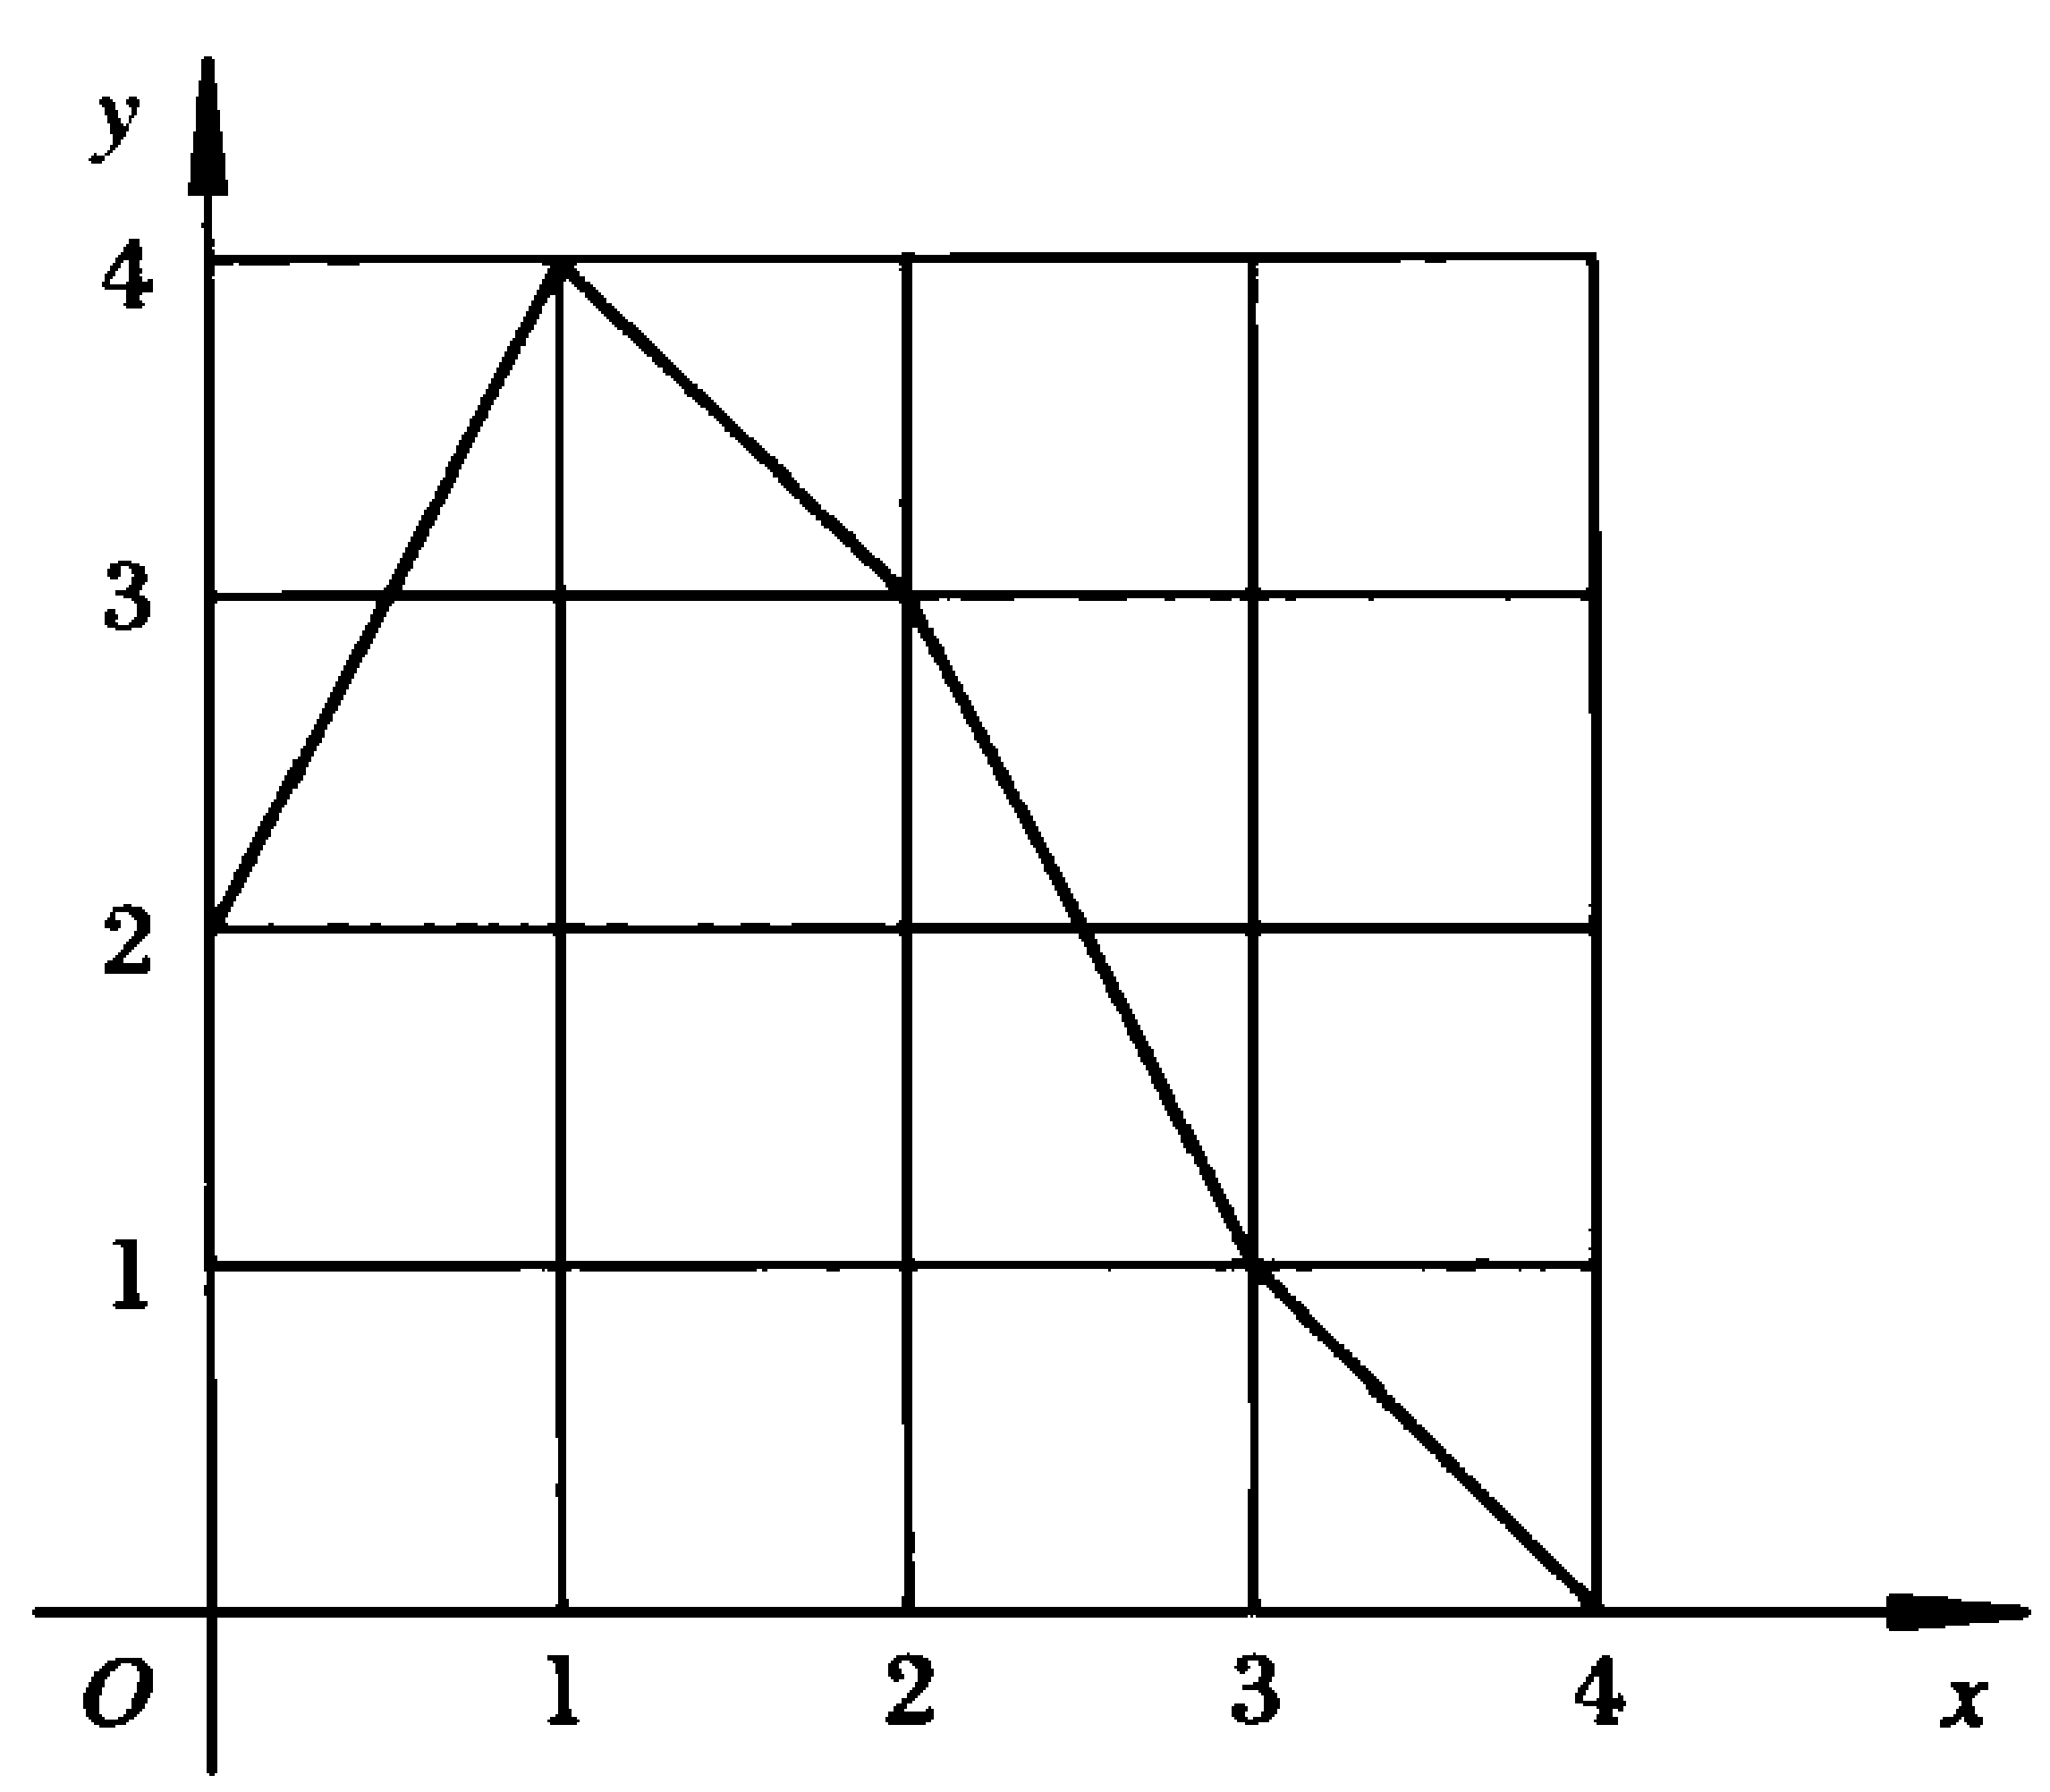
\includegraphics[width=0.43\linewidth]{figures/fig_2_176_1.png}\end{center}
\end{minipage}\par\vfill
\newpage
\noindent\begin{minipage}{\textwidth}\ProblemHeading{习题}{2.177}
设 $f:I\to I$，记 $f^{\circ n}$ 为 $f$ 的 $n$ 次复合；若 $n$ 是使 $f^{\circ n}(x)=x$ 成立的最小正整数，则称 $x$ 为 $n$ 周期点。若 $x$ 是一个 $n$ 周期点，记 $x_0=x$、$x_k=f^{\circ k}(x)$（$1\le k<n$）。证明周期轨道中的点 $x_0,\ldots,x_{n-1}$ 两两不同，且每个都是 $f$ 的 $n$ 周期点。
\end{minipage}\par\vfill
\noindent\begin{minipage}{\textwidth}\ProblemHeading{习题}{2.178}
设 $f:[a,b]\to[a,b]$ 连续，记 $f^{\circ n}$ 为 $f$ 的 $n$ 次复合；若 $n$ 是使 $f^{\circ n}(x)=x$ 成立的最小正整数，则称 $x$ 为 $n$ 周期点。若 $f$ 有4周期点，证明 $f$ 必有2周期点。
\end{minipage}\par\vfill
\noindent\begin{minipage}{\textwidth}\ProblemHeading{习题}{2.179}
设 $f:[a,b]\to[a,b]$ 连续，记 $f^{\circ n}$ 为 $f$ 的 $n$ 次复合；若 $n$ 是使 $f^{\circ n}(x)=x$ 成立的最小正整数，则称 $x$ 为 $n$ 周期点。若对某个正整数 $n$，$f$ 有 $2^n$ 周期点，证明对每个 $1\le k<n$，$f$ 都有 $2^k$ 周期点。
\end{minipage}\par\vfill
\newpage
\noindent\begin{minipage}{\textwidth}\ProblemHeading{习题}{2.180}
设 $I$ 为区间，$f:I\to I$ 连续，$I_0,I_1,\ldots,I_n$ 为 $I$ 的非空闭子区间，且 $f(I_i)\supseteq I_{i+1}$（$0\le i<n$）。证明存在 $x\in I_0$，使 $f^{\circ i}(x)\in I_i$（$1\le i\le n$），其中 $f^{\circ i}$ 表示 $i$ 次复合。
\end{minipage}\par\vfill
